%Version 3.1 December 2024
% See section 11 of the User Manual for version history
%
%%%%%%%%%%%%%%%%%%%%%%%%%%%%%%%%%%%%%%%%%%%%%%%%%%%%%%%%%%%%%%%%%%%%%%
%%                                                                 %%
%% Please do not use \input{...} to include other tex files.       %%
%% Submit your LaTeX manuscript as one .tex document.              %%
%%                                                                 %%
%% All additional figures and files should be attached             %%
%% separately and not embedded in the \TeX\ document itself.       %%
%%                                                                 %%
%%%%%%%%%%%%%%%%%%%%%%%%%%%%%%%%%%%%%%%%%%%%%%%%%%%%%%%%%%%%%%%%%%%%%

%%\documentclass[referee,sn-basic]{sn-jnl}% referee option is meant for double line spacing

%%=======================================================%%
%% to print line numbers in the margin use lineno option %%
%%=======================================================%%

%%\documentclass[lineno,pdflatex,sn-basic]{sn-jnl}% Basic Springer Nature Reference Style/Chemistry Reference Style

%%=========================================================================================%%
%% the documentclass is set to pdflatex as default. You can delete it if not appropriate.  %%
%%=========================================================================================%%

%%\documentclass[sn-basic]{sn-jnl}% Basic Springer Nature Reference Style/Chemistry Reference Style

%%Note: the following reference styles support Namedate and Numbered referencing. By default the style follows the most common style. To switch between the options you can add or remove �Numbered� in the optional parenthesis. 
%%The option is available for: sn-basic.bst, sn-chicago.bst%  
 
%%\documentclass[pdflatex,sn-nature]{sn-jnl}% Style for submissions to Nature Portfolio journals
%%\documentclass[pdflatex,sn-basic]{sn-jnl}% Basic Springer Nature Reference Style/Chemistry Reference Style
\documentclass[pdflatex,sn-mathphys-num]{sn-jnl}% Math and Physical Sciences Numbered Reference Style
%%\documentclass[pdflatex,sn-mathphys-ay]{sn-jnl}% Math and Physical Sciences Author Year Reference Style



%%\documentclass[pdflatex,sn-aps]{sn-jnl}% American Physical Society (APS) Reference Style
%%\documentclass[pdflatex,sn-vancouver-num]{sn-jnl}% Vancouver Numbered Reference Style
%%\documentclass[pdflatex,sn-vancouver-ay]{sn-jnl}% Vancouver Author Year Reference Style
%%\documentclass[pdflatex,sn-apa]{sn-jnl}% APA Reference Style
%%\documentclass[pdflatex,sn-chicago]{sn-jnl}% Chicago-based Humanities Reference Style

%%%% Standard Packages
%%<additional latex packages if required can be included here>
% 设置中文


\RequirePackage{etex}

\usepackage[UTF8]{ctex}
% \usepackage{xeCJK}
% \setCJKmainfont{Noto Serif CJK SC}
% \usepackage{unicode-math}   % 替代 amssymb + bm + fontspec

\usepackage{subfigure}
\usepackage{tabularx}
\usepackage{graphicx}
\usepackage{float}
\usepackage{epstopdf}
\usepackage{microtype}
\usepackage{enumitem}
\usepackage{multirow}
\usepackage{bbding}
\usepackage{amsmath}
% \usepackage{color}
\usepackage{bm}
\usepackage{cleveref}  
% \usepackage[authoryear,sort&compress,longnamesfirst]{natbib}
\usepackage{xcolor}
\usepackage{hyperref}
\usepackage{amssymb} 
\usepackage{amsthm} 
\usepackage{booktabs}
%%%%
% 可选:让 epstopdf 自动在 \includegraphics 时启用
\epstopdfsetup{outdir=./}
%%%%%=============================================================================%%%%
%%%%  Remarks: This template is provided to aid authors with the preparation
%%%%  of original research articles intended for submission to journals published 
%%%%  by Springer Nature. The guidance has been prepared in partnership with 
%%%%  production teams to conform to Springer Nature technical requirements. 
%%%%  Editorial and presentation requirements differ among journal portfolios and 
%%%%  research disciplines. You may find sections in this template are irrelevant 
%%%%  to your work and are empowered to omit any such section if allowed by the 
%%%%  journal you intend to submit to. The submission guidelines and policies 
%%%%  of the journal take precedence. A detailed User Manual is available in the 
%%%%  template package for technical guidance.
%%%%%=============================================================================%%%%

%% as per the requirement new theorem styles can be included as shown below
\theoremstyle{thmstyleone}%
\newtheorem{theorem}{Theorem}%  meant for continuous numbers
%%\newtheorem{theorem}{Theorem}[section]% meant for sectionwise numbers
%% optional argument [theorem] produces theorem numbering sequence instead of independent numbers for Proposition
\newtheorem{proposition}[theorem]{Proposition}% 
%%\newtheorem{proposition}{Proposition}% to get separate numbers for theorem and proposition etc.
\newtheorem{lemma}{Lemma}[section] 
\newtheorem{assumption}{Assumption}
\theoremstyle{thmstyletwo}%
\newtheorem{example}{Example}%
\newtheorem{remark}{Remark}%

\theoremstyle{thmstylethree}%
\newtheorem{definition}{Definition}%

\raggedbottom
%%\unnumbered% uncomment this for unnumbered level heads

\begin{document}

\title[Article Title]{Predefined Time Prescribed Performance Backstepping Control for Robotic Manipulators with Input Saturation}

%%=============================================================%%
%% GivenName	-> \fnm{Joergen W.}
%% Particle	-> \spfx{van der} -> surname prefix
%% FamilyName	-> \sur{Ploeg}
%% Suffix	-> \sfx{IV}
%% \author*[1,2]{\fnm{Joergen W.} \spfx{van der} \sur{Ploeg} 
%%  \sfx{IV}}\email{iauthor@gmail.com}
%%=============================================================%%

\author[1,2]{\fnm{} \sur{Shuli Liu}}\email{shunnee@163.com}
% \credit{Writing - Original Draft, Methodology, Software, Visualization, Data curation}


\author*[3]{\fnm{} \sur{Yi Liu}}\email{liuyi_hust@163.com}
\author*[3]{\fnm{} \sur{Jingang Liu}}\email{wellbuild@126.com}
% \credit{Resources, Investigation, Formal analysis, Conceptualization, Writing - Review \& Editing}
% \equalcont{These authors contributed equally to this work.}

% \credit{Project administration, Validation, Funding acquisition, Writing - Review \& Editing}
% \equalcont{These authors contributed equally to this work.}
\author*[1,2]{\fnm{} \sur{Yin Yang}}\email{yangyinxtu@xtu.edu.cn}
% \credit{Supervision, Funding acquisition, Writing - Review \& Editing}
% \equalcont{These authors contributed equally to this work.}

\affil[1]{\orgname{School of Mathematics and Computational Science, Xiangtan University}, \orgaddress{\street{Street}, \city{City}, \postcode{411105}, \country{China}}}

\affil[2]{\orgname{National Center for Applied Mathematics in Hunan}, \orgaddress{\street{Street}, \city{City}, \postcode{411105}, \country{China}}}

\affil[3]{\orgname{School of Mechanical Engineering and Mechanics, Xiangtan University}, \orgaddress{\street{Street}, \city{City}, \postcode{411105}, \country{China}}}



% Here goes the abstract
\abstract{
% To simultaneously address the challenges of uncontrollable convergence time and the difficulty of unifying performance constraints in trajectory tracking control for uncertain nonlinear robotic manipulators, this paper proposes a novel adaptive control framework that integrates predefined-time convergence with prescribed performance constraints. Specifically, a new class of Bernstein-polynomial-based performance functions is designed to achieve smooth and adjustable boundaries for both position and velocity errors, significantly reducing dependence on initial error conditions. An exponential barrier Lyapunov function is further introduced to strictly constrain the entire error evolution process. The controller is constructed using the backstepping method and incorporates a radial basis function neural network for online compensation of unknown nonlinear dynamics, thereby enhancing the system’s adaptability and robustness. The proposed approach organically combines predefined-time stability theory with dynamic performance regulation, theoretically guaranteeing the uniform boundedness of all closed-loop signals and prescribed-time convergence of the tracking error. Finally, simulation and experimental verification are carried out on a typical two-degree-of-freedom robotic arm system and a real six-degree-of-freedom collaborative robot platform. The results show that the proposed method outperforms existing schemes in terms of tracking accuracy, convergence speed and robustness, and is particularly suitable for high-performance and time-sensitive robotic systems.
本文研究了具有未知动力学、有界扰动以及执行器饱和条件下的机器人机械臂轨迹跟踪控制问题,提出了一种立于任何初始状态条件的预定义时间预设性能约束的自适应反步控制方法。针对传统预设性能控制中存在的初值奇异性和误差变换非光滑问题,针对每个通道独立设计了结合多项式性能函数与误差缩放函数的预定义时间误差变换结构,确保系统状态在预定义时间内严格且平滑地满足全局预设性能约束。
为处理反步控制及执行器饱和输入引起的计算复杂度爆炸问题,设计了一种预定义时间饱和补偿器,以同时消除命令滤波与输入饱和的不利影响。此外,引入一阶滑模扰动观测器实时估计并补偿系统中未知的有界扰动,利用径向基函数神经网络对系统未建模动态进行辨识和补偿,从而提高了控制系统的鲁棒性和跟踪精度。同时,结合预定义时间理论和自适应动态障碍李雅普诺夫函数,严格证明了闭环系统在预定义时间内的全局稳定性和误差收敛性。
数值和实验结果结果验证了所提出方法的有效性,与现有方法相比,本文方法在响应速度、稳态精度及鲁棒性能方面表现出明显优势。

}
\keywords{Prescribed performance control, predefined-time stability, adaptive dynamic barrier Lyapunov function, backstepping control, input saturation, robotic manipulators' trajectory tracking.
}
\maketitle


\section{Global prescribed–performance function}

为同时实现“\emph{初值全局可行}、\emph{预定义时间内平滑收紧}”与“\emph{收敛后对饱和/扰动的自适应友好}”,构造一类全局预设性能函数(G-PPF),系统性解决传统 PPC/BLF-PPF 的三类痛点:(\emph{i}) 初值越界诱发进入阶段奇异,常需投影/重置/非对称缩放等权宜处理;(\emph{ii}) 在 $T_p$ 处边界多为仅连续非 $C^1$,易在控制律中产生尖峰项并放大噪声;(\emph{iii}) 收敛后采用固定且过窄管径,面对执行器饱和与外扰时保守与抖振并存。所提 G-PPF 以核函数 $\phi(b)=-\ln b$ 与光滑窗 $s(b)$ 协同保证 $\rho(0^+)=+\infty$ 与 $\dot\rho(T_p^-)=0$,实现“\emph{预定义时间内平滑收紧而初值全局合法}”。进一步,引入\emph{前段缩放} $\sigma(t)$(调速收紧)与\emph{后段“呼吸式”缩放} $\Sigma(t)$(稳态放宽)两级解耦调节,并按饱和残差与扰动强度低通自适应调整约束,避免长期保守。与此同时,给出 $\dot\rho(t)$ 的显式解析式,使 BLF 导数中的边界变化项可被严格抵消,不遗留常数残差,从而将闭环 Lyapunov 不等式自然规范为 PTS-ISS 形态。该构造与反步、饱和补偿、RBFNN 等模块无缝兼容,可在严格保证预定义时间稳定的同时提升稳态精度与执行器友好性。

\subsection{Definition}

令 $T_p>0$ 为预定义收敛时间、$0<p<1$,定义归一化时间

$$
b(t)=\bigl(t/T_p\bigr)^p\in(0,1],\qquad \dot b=\tfrac{p}{T_p}\bigl(t/T_p\bigr)^{p-1}>0,
$$

取 $C^1$ 光滑窗
\begin{equation}\label{eq\:gppf-window}
s(b)=1-3b^2+2b^3,\quad s(0)=1,\ s(1)=0,\ s'(1)=0,
\end{equation}
以及全局核函数
\begin{equation}\label{eq\:gppf-kernel}
\phi(b)=-\ln b,\qquad \phi(b)\to+\infty\ (b\to0^+),\ \ \phi(1)=0.
\end{equation}
对每个通道 $i=1,\dots,n$,定义全局性能函数
\begin{equation}\label{eq\:gppf-def}
\rho_i(t)=
\begin{cases}
\displaystyle a+\sigma_i(t),\phi!\left(b(t)\right),s!\left(b(t)\right), & 0<t<T_p,\\
\displaystyle a\bigl[1+g(t),\Sigma_i(t)\bigr], & t\ge T_p,
\end{cases}
\end{equation}
其中 $a>0$ 表示稳态精度下界。$\sigma_i(t)$ 调节 $t<T_p$ 阶段的\emph{收紧速率},$\Sigma_i(t)$ 则在 $t\ge T_p$ 阶段实现\emph{呼吸式放宽}以顺应饱和与扰动:
\begin{align}
&\sigma_i(t)=\operatorname{Proj}*{[\sigma*{\min},,\sigma_{\max}]}!\Bigl(\sigma_{i0}+k_u r_{u,i}+k_d r_{d,i}\Bigr),\label{eq\:gppf-sigma}\\
&\tau_u \dot r_{u,i}=-r_{u,i}+|\Delta u_i|,\qquad
\tau_d \dot r_{d,i}=-r_{d,i}+|d_i|,\nonumber
\end{align}
其中 $\sigma_{i0},k_u,k_d,\tau_u,\tau_d>0$,$\Delta u_i=u_i-\operatorname{sat}(u_i)$ 为饱和残差。$t\ge T_p$ 时,以 $C^1$ 门控函数确保光滑拼接:
\begin{equation}\label{eq\:gppf-gate}
g(t)=1-\exp!\bigl(-\iota (t-T_p)^2\bigr),\quad \iota>0,\ \ g(T_p)=0,\ g'(T_p)=0,
\end{equation}
并设呼吸幅值
\begin{align}
&\Sigma_i(t)=\operatorname{Proj}*{[,0,,\Sigma*{\max},]}!\Bigl(k_u r_{u,i}+k_d r_{d,i}+k_e r_{e,i}\Bigr),\label{eq\:gppf-Sigma}\\
&\tau_e \dot r_{e,i}=-r_{e,i}+|e_i|,\qquad k_e,\tau_e>0.\nonumber
\end{align}

\subsection{Derivatives for exact compensation}

由 $\phi'(b)=-1/b$、$s'(b)=-6b+6b^2$ 与 \cref{eq:gppf-window}–\cref{eq:gppf-def},在 $0<t<T_p$ 有
\begin{equation}\label{eq\:gppf-drho-pre}
\dot\rho_i
= \dot\sigma_i,\phi(b),s(b)
* \sigma_i\Bigl[\phi'(b),s(b)+\phi(b),s'(b)\Bigr]\dot b .
  \end{equation}
  在 $t\ge T_p$,
  \begin{equation}\label{eq:gppf-drho-post}
  \dot\rho_i
  = a\Bigl[g'(t),\Sigma_i(t)+g(t),\dot\Sigma_i(t)\Bigr],\qquad
  \dot\Sigma_i=\text{Proj-grad}\Bigl(k_u\dot r_{u,i}+k_d\dot r_{d,i}+k_e\dot r_{e,i}\Bigr).
  \end{equation}
  在 BLF 框架中,诸如 $\dot V_{\mathrm{BLF}}\ni (\dot\rho_i \rho_i)\cdot(\cdot)$ 的边界变化项可用 \cref{eq:gppf-drho-pre,eq:gppf-drho-post} 精确抵消,避免残余常数项,便于将闭环不等式规范为 PTS-ISS 形式。

\subsection{Properties}

% \begin{properties}
对 $\rho_i(t)$ 于 \cref{eq:gppf-def}–\cref{eq:gppf-Sigma},成立:
\begin{enumerate}
\item \textbf{全局初值合法性:} $\displaystyle\lim_{t\to0^+}\rho_i(t)=+\infty$,故任意有限 $e_i(0)$ 均满足 $|e_i(0)|<\rho_i(0^+)$。
\item \textbf{预定义时间收紧与 $C^1$ 拼接:} 由 $\phi(1)=0$、$s(1)=0$ 得 $\rho_i(T_p^-)=a$;由 $s'(1)=0$ 与 $g(T_p)=g'(T_p)=0$ 得 $\dot\rho_i(T_p^-)=\dot\rho_i(T_p^+)=0$,实现 $C^1$ 级平滑衔接。
\item \textbf{单调与平滑($0<t\le T_p$):} 在 $\dot\sigma_i\le 0$(或 $\dot\sigma_i$ 由低通滤波器充分抑制)时,\cref{eq:gppf-drho-pre} 第二项严格为负,且第一项不为正,故 $\rho_i(t)$ 在 $(0,T_p]$ 上严格递减且 $C^1$。更一般地,只要 $|\dot\sigma_i|$ 足够小,单调性仍保持。
\item \textbf{$t\ge T_p$ 的自适应稳态友好性:} $\rho_i(t)=a,[1+g(t)\Sigma_i(t)]\ge a$,其中 $g$、$\Sigma_i$ 有界且经低通滤波,保证边界正性与缓变性;$\Sigma_i$ 随饱和残差与扰动强度自适应调整,可在不破坏约束的前提下降低保守性。
\item \textbf{实现友好的导数:} \cref{eq:gppf-drho-pre}–\cref{eq:gppf-drho-post} 给出闭式导数,便于在 BLF 导数中做\emph{精确补偿},避免由未知边界变化引入的保守加项。
\end{enumerate}
% \end{properties}

\begin{remark}[Parameter guidelines and compatibility]
\emph{参数选取与实现建议:} 令 $\sigma_{\min}\le\sigma_{i0}\le\sigma_{\max}$,并取 $0\le\Sigma_{\max}\le 0.5$ 将收敛后最大放宽幅度限制在 $50%$ 以内;选 $\tau_u,\tau_d,\tau_e$ 相对较大以平缓 $\rho_i(t)$ 变化,避免激发闭环;优先设置 $k_u,k_d\gg k_e$,使“呼吸”主要由饱和/扰动而非瞬态误差驱动;$p\in(0,1)$ 决定早期收紧速率,$p\to 1$ 较温和、$p\to 0$ 较迅猛,可与 $\sigma_{i0}$ 联合整定。实现上,$\operatorname{Proj}$ 与其“Proj-grad”在投影边界处按 Carathéodory/几乎处处可导理解,常规数值实现取“饱和即停”的次梯度即可稳定工作。\emph{兼容性:} 该 G-PPF 为控制器无关的上层约束构件,可与反步、非线性抗饱和补偿、RBFNN 动态补偿及滑模/积分增强等模块直接耦合,且保持 PTS-ISS 证法的闭式推导。
\end{remark}

\begin{figure}[H]
\centering
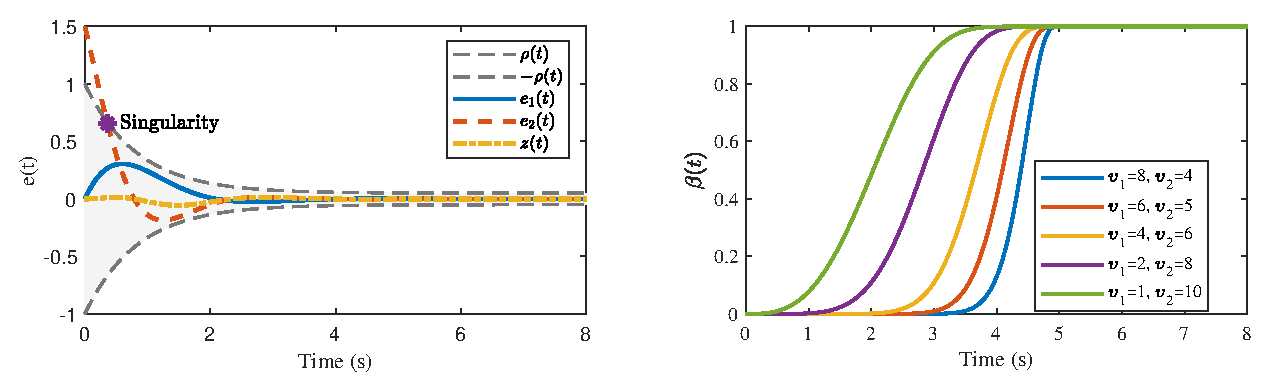
\includegraphics[width=0.9\textwidth]{fig1.eps}
\caption{全局动态 G-PPF:预定义时间内平滑收紧与收敛后“呼吸式”放宽。}
\label{fig:1}
\end{figure}

---

\noindent\textbf{与原稿相比的关键改进要点:}(1)动机与三类痛点更聚焦,建立到设计要素的“一一对应”;(2)显式强调 $C^1$ 拼接与 BLF 导数的“精确补偿”关系,服务于后续 PTS-ISS 证明链;(3)单调性给出可操作的充分条件($\dot\sigma_i\le 0$ 或“足够小”);(4)参数整定与实现细节(Proj-grad、$p$ 的物理含义)前置,降低读者复现实践门槛;(5)行文删繁就简,保留必要数学细节与工程语义。










\subsection{System description}



求$V_1$ 的时间导数为
\begin{equation}\label{eq:25}
	\begin{aligned}
\dot V_1
&=\sum_{i=1}^{n}\left[
\frac{\rho_{1,i}^4\,z_{1,i}}{\big(\rho_{1,i}^{2}-z_{1,i}^{2}\big)^{2}}\dot z_{1,i}
-
\frac{\rho_{1,i}\,z_{1,i}^{4}}{\big(\rho_{1,i}^{2}-z_{1,i}^{2}\big)^{2}}\dot \rho_{1,i}
\right]\\
% &=\sum_{i=1}^{n}\left[
% \frac{\rho_{1,i}^4\,z_{1,i}}{\big(\rho_{1,i}^{2}-z_{1,i}^{2}\big)^{2}}(z_{2,i}-\dot q_{d,i}+\alpha^{f}_i+\zeta_i)-
% \frac{\rho_{1,i}\,z_{1,i}^{4}}{\big(\rho_{1,i}^{2}-z_{1,i}^{2}\big)^{2}}\dot \rho_{1,i}
% \right]
\end{aligned}
\end{equation}

记
$
P_{j,i}=\frac{\rho_{j,i}^4}{(\rho_{j,i}^2-z_{j,i}^2)^2}>0,
Q_{j,i}=\frac{ z_{j,i}^4}{(\rho_{j,i}^2-z_{j,i}^2)^2}>0,
\Phi_{j,i}=\frac{z_{j,i}\left(\rho_{j,i}^{2}-z_{j,i}^{2}\right)}{\rho_{j,i}^{4}}=\frac{z_{j,i}(\rho_{j,i}^2-z_{j,i}^2)}{P_{j,i}}, j\in\{1,2\}
$,
$\dot z_{1,i}= z_{2,i}-\dot q_{d,i}+\alpha^{f}_i+\zeta_i$, 将它们代入 BLF 导数后,并根据公式(),得到
$$
\dot V_1=\sum_{i=1}^n\!\Big[P_{1,i} z_{1,i}z_{2,i}+P_{1,i}z_{1,i}(\alpha_i+\zeta_i-\dot q_{d,i})-P_{1,i}z_{1,i}\tilde\alpha_i-Q_{1,i}\rho_{1,i} \dot\rho_{1,i}\Big]
$$

Let ${V_{j,i}}=\frac{1}{2}\frac{\rho_{j,i}^2 z_{j,i}^2}{\rho_{j,i}^2-z_{j,i}^2}, \Psi(V_{j,i})=\frac{\pi}{ \eta T_p}\Big((V_{j,i})^{\,1-\eta/2}+n^{-\frac{\eta}{2} }(V_{j,i})^{\,1+\eta/2}\Big)$, 我们设计
$$
\mathcal{K}_{1,i}(z_{j,i},\rho_{j,i})
=\frac{\rho_{j,i}^2}{2}\frac{\Psi(V_{j,i})}{V_{j,i}}
=\frac{\pi\,\rho_{j,i}^2}{2\eta T_p}\Big((V_{j,i})^{-\eta/2}+n^{-\frac{\eta}{2} }(V_{j,i})^{\eta/2}\Big).
$$

把它代回,可设计虚拟控制律为:
\begin{equation}\label{eq:25}
\alpha_i = \dot q_{d,i}-\zeta_i+\frac{z_{1,i}^3}{\rho_{1,i}^3}\,\dot\rho_{1,i}
-\mathcal{K}_{1,i}(z_{1,i},\rho_{1,i})\Phi_{1,i}
-k_{1,i} \rho_{1,i}^2 \Phi_{1,i},
\end{equation}
where $k_1=\mathrm{diag}\{k_{1,1},k_{1,i},\cdots,k_{1,n}\}>0$, $k_{1,i}>0$,

则一步 Lyapunov 导数化简为

$$
\dot V_1
\le \sum_{i=1}^n \Big[ P_{1,i}z_{1,i} z_{2,i}
-\Psi(V_{1,i})-P_{1,i}z_{1,i}\tilde\alpha_i- k_{1,i}\frac{\rho_{1,i}^2 z_{1,i}^2}{\rho_{1,i}^2-z_{1,i}^2} 
\Big].
$$


In the second step, a BLF is used as an energy function for the error dynamics. We choose:
\begin{equation}\label{eq:25}
	V_2= \frac{1}{2}\sum_{i=1}^{n} \frac{\rho_{2,i}^2 z_{2,i}^2}{\rho_{2,i}^2-z_{2,i}^2}. 
\end{equation}


Using $\dot z_{2,i}=\dot x_{2,i}-\dot\alpha_i^{f}-\dot\zeta_i$, we obtain the time derivative of $V_2$ is as
\begin{equation}
	\begin{aligned}
		\dot V_2& = \sum_{i=1}^n \Big[\,P_{2,i}z_{2,i}\,(\dot x_{2,i}-\dot\alpha_i^{f}-\dot\zeta_i)-Q_{2,i}\rho_{2,i}\,\dot\rho_{2,i}\,\Big]\\
		&
		 = \sum_{i=1}^n \left[\,P_{2,i}z_{2,i}\,\left(f_i(x)+h_i(x,t)+g_i(u_i-\Delta u_i)+d'(t)-\dot\alpha_i^{f}-\delta_i\ +\ \mu_2\,\zeta_i\ +\ g_i\,\Delta u_i-\tfrac{z_{2}^{3}}{\rho_{2,i}^{3}}\dot\rho_{2,i} \right)\right]
	\end{aligned}
\end{equation}

Let $Q_2=\mathrm{col}\{Q_{2,i}\}$,
$P_1=\mathrm{col}\{P_{1,i}\}$,
$\Phi_2=\mathrm{col}\{\Phi_{2,i}\}$. The control input torque is designed as
\begin{equation}\label{eq:tau-cmd}
\begin{aligned}
u =&C(q,\dot{q})x_2 + G(q)\\
&+M(q)\left[\dot\alpha^{f}+\delta -\mu_2\,\zeta-\frac{P_1}{P_2}z_1+\tfrac{z_{2}^{3}}{\rho_{2,i}^{3}}\dot\rho_{2,i}-\mathcal{K}_{2}(z_{2},\rho_{2,i}) \Phi_{2}
-\hat{h}(\chi)
-\hat \omega
-k_s\,\mathrm{sgn}(z_{2})-k_{2}\rho_{2,i}^2 \Phi_{2,i}\right]
\end{aligned}
\end{equation}


where $k_2=\mathrm{diag}\{k_{2,1},k_{2,i},\cdots,k_{2,n}\}>0$, $k_{2,i}>0$, $k_s>0$.

Let $\chi=\{q,\dot{q}\}\in\mathbb{R}^m$ be the regressor and $\psi(\chi)\in\mathbb{R}^{N}$ the normalized basis. Approximate the structured uncertainty by 
\( \hat h_i(\chi)=\hat \theta_i^\top \psi_i(\chi)\),
with $\theta_i\in\mathbb{R}^{N}  $ adapted online by
\begin{equation}\label{eq:theta-law}
\dot{\hat{\theta}}_i = \varrho_i\,P_{2,i} z_{2,i}\psi(\chi) - \kappa_i\,\hat{\theta}_i,\qquad
\varrho_i,\kappa_i>0.
\end{equation}

% 将外扰的项定义为
% $\omega(x,t)= M^{-1}(q) d(t)$。
将结构不确定估计误差和外扰的剩余项定义为
$\omega(x,t)=h(x)-\hat h(\chi)+ M^{-1}(q) d(t)$。

为避免直接微分速度,采用一阶跟踪微分器作为观测器
\begin{equation}
	\begin{cases}
\dot\vartheta =-\omega_d\,\vartheta+\omega_d\,x_2,  \\
\hat{\dot x}_2=\omega_d(x_2-\vartheta),   \\
\dot{\hat \omega}= -\Lambda_o\,\hat \omega
+\Lambda_o\left(\hat{\dot x}_2 - f(x) - M^{-1}(q)\,\mathrm{sat}(u) - \hat h(\chi)\right),
\end{cases}
\end{equation}
where $\Lambda_o=\mathrm{diag}\{\lambda_{o,i}\}>0, \omega_d>0, \vartheta(0)=x_2(0), \hat \omega(0)=0$,
设观测误差为 $\tilde \omega=\omega-\hat\omega$. 其动力学为

$$
\dot{\tilde\omega}
= -\Lambda_o\,\tilde\omega\;+\;\Delta_\omega,\qquad
\Delta_\omega:=\dot\omega-\Lambda_o\,\varepsilon_d,
$$
where $\Lambda_o=\mathrm{diag}\{\lambda_{o,i}\}>0, w_d>0, \vartheta(0)=x_2(0)$,$\varepsilon_d:=\hat{\dot x}_2-\dot x_2$ 为跟踪微分器误差。


根据公式可得到
\begin{equation}
	\begin{aligned}
	\dot V_2
\le&+\sum_{i=1}^n \left( - k_{2,i}\frac{\rho_{2,i}^2 z_{2,i}^2}{\rho_{2,i}^2-z_{2,i}^2}-\Psi(V_{2,i})-P_{2,i}z_{2,i}\tilde{\omega}_i  \right) -k_s\sum_{i=1}^n P_{2,i} \left\lvert z_{2,i}\right\rvert
\end{aligned}
\end{equation}








\begin{equation}\label{eq:45}
	\begin{aligned}
		\dot{V} \le&\sum_{i=1}^n \left( - k_{1,i}\frac{\rho_{1,i}^2 z_{1,i}^2}{\rho_{1,i}^2-z_{1,i}^2}-\Psi(V_{1,i})-P_{1,i}z_{1,i}\tilde\alpha_i\right)
		+\sum_{i=1}^n \left( - k_{2,i}\frac{\rho_{2,i}^2 z_{2,i}^2}{\rho_{2,i}^2-z_{2,i}^2}-\Psi(V_{2,i})-P_{2,i}z_{2,i}\tilde{\omega}_i  \right)\\
		& -k_s\sum_{i=1}^n P_{2,i} \left\lvert z_{2,i}\right\rvert +\tilde\alpha^\top \dot{\tilde \alpha}+\tilde \omega^\top \dot{\tilde \omega}+\sum_{i=1}^n\tfrac{1}{\varrho_i}\tilde \theta_i^\top \dot{\tilde \theta}_i \\
		\le&\sum_{i=1}^n \left( - k_{1,i}\frac{\rho_{1,i}^2 z_{1,i}^2}{\rho_{1,i}^2-z_{1,i}^2}-\Psi(V_{1,i})\right)
		+\sum_{i=1}^n \left( - k_{2,i}\frac{\rho_{2,i}^2 z_{2,i}^2}{\rho_{2,i}^2-z_{2,i}^2}-\Psi(V_{2,i})  \right)\\
		& -\sum_{i=1}^nP_{2,i}z_{2,i}\tilde{\omega}_i +\tilde \omega^\top \dot{\tilde \omega}-k_s\sum_{i=1}^n P_{2,i} \left\lvert z_{2,i}\right\rvert+\tilde\alpha^\top \dot{\tilde \alpha}-\sum_{i=1}^n P_{1,i}z_{1,i}\tilde\alpha_i+\sum_{i=1}^n\tfrac{1}{\varrho_i}\tilde \theta_i^\top \dot{\tilde \theta}_i 
	\end{aligned}
\end{equation}

$$
\rho_{2,i}^2 - z_{2,i}^2 \le \rho_{2,i}^2
$$



Let 
$$
\mathcal{L} =-\sum_{i=1}^nP_{2,i}z_{2,i}\tilde{\omega}_i\;+\;\tilde \omega^\top \dot{\tilde \omega}\;-\;k_s\sum_{i=1}^n P_{2,i} | z_{2,i} |
$$


利用不等式 $ab\le k\,a+\frac{b^2}{4k}$($(\sqrt{k\,a}-\frac{b}{2\sqrt{k}})^2\ge0$)并取
$a=P_{2,i}|z_{2,i}|,\ b=|\tilde\omega_i|,\ k=k_s$,对每个通道有

$$
-\,P_{2,i}z_{2,i}\tilde\omega_i
\ \le\
P_{2,i}|z_{2,i}|\,|\tilde\omega_i|
\ \le\
k_s P_{2,i}|z_{2,i}|+\frac{1}{4k_s}\tilde\omega_i^{\,2}.
$$

于是

$$
-\,k_s\!\sum_{i=1}^n\! P_{2,i}|z_{2,i}|
-\sum_{i=1}^n P_{2,i}z_{2,i}\tilde\omega_i
\ \le\
\frac{1}{4k_s}\,\|\tilde\omega\|^2
$$


由观测器误差$
\dot{\tilde\omega}= -\Lambda_o\,\tilde\omega+\Delta_\omega,
\Lambda_o=\mathrm{diag}\{\lambda_{o,i}\}>0$, 并根据Young不等式得

$$
\tilde\omega^\top\dot{\tilde\omega}
= -\tilde\omega^\top\Lambda_o\tilde\omega+\tilde\omega^\top\Delta_\omega
\ \le\
-\tilde\omega^\top\Lambda_o\tilde\omega
+\frac{\varepsilon}{2}\tilde\omega^\top\Lambda_o\tilde\omega
+\frac{1}{2\varepsilon}\Delta_\omega^\top\Lambda_o^{-1}\Delta_\omega \le\
-\Big(1-\tfrac{\varepsilon}{2}\Big)\tilde\omega^\top\Lambda_o\tilde\omega
+\frac{1}{2\varepsilon}\big\|\Lambda_o^{-1/2}\Delta_\omega\big\|^2,
$$



把(A)与(B)相加:

$$
\begin{aligned}
	\mathcal{L}
&\le
-\Big(1-\tfrac{\varepsilon}{2}\Big)\tilde\omega^\top\Lambda_o\tilde\omega
+\frac{1}{4k_s}\|\tilde\omega\|^2
+\frac{1}{2\varepsilon}\big\|\Lambda_o^{-1/2}\Delta_\omega\big\|^2.
\end{aligned}
$$

利用 $\tilde\omega^\top\Lambda_o\tilde\omega\ge \lambda_{o,\min}\|\tilde\omega\|^2$,得到

$$
\mathcal{L} \le\
-\Big(\big(1-\tfrac{\varepsilon}{2}\big)\lambda_{o,\min}-\tfrac{1}{4k_s}\Big)\|\tilde\omega\|^2
+\frac{1}{2\varepsilon}\big\|\Lambda_o^{-1/2}\Delta_\omega\big\|^2.
$$

令 $\varepsilon=\tfrac12$(简洁且常用),净负系数为 $\tfrac{3}{4}\lambda_{o,\min}-\tfrac{1}{4k_s}$。
只要$
\boxed{ \ k_s\;>\;\frac{1}{3\,\lambda_{o,\min}}\ }$

 $\frac{1}{2\varepsilon}\|\Lambda_o^{-1/2}\Delta_\omega\|^2$ 作为输入项(由 $\Delta_\omega=\dot\omega-\Lambda_o\varepsilon_d$ 决定)并入 $\sigma(\|r(t)\|)$。

% ---

%  融入总 Lyapunov 导数与 PTS–ISS

% 将(C)代入总 $\dot V$,并与一步/二步 BLF 的主衰减项
% $-\Psi(S_{j,i})$、$-k_{j,i}\frac{\rho_{j,i}^2 z_{j,i}^2}{\rho_{j,i}^2-z_{j,i}^2}$ 合并,再用幂和不等式把 $\sum_i\Psi(S_{j,i})$ 下界为 $V$ 的函数,可得

% $$
% \dot V
% \ \le\
% -\frac{\pi}{\eta T_p^\star}\big(V^{1-\eta/2}+V^{1+\eta/2}\big)
% \ -\ c_\omega\|\tilde\omega\|^2
% \ +\ \sigma(\|r(t)\|),
% $$

% 其中 $c_\omega=\tfrac{3}{4}\lambda_{o,\min}-\tfrac{1}{4k_s}>0$。这正是你需要的 **PTS–ISS** 标准形式。












































% 其中 $\odot$ 表示Hadamard积。
% % 特别地,取 $\varepsilon_1=\varepsilon_2=\tfrac12$ 时,

% % \begin{equation}\label{eq:45}
% % 	\begin{aligned}
% % \mathcal T
% % \le 
% % &-\tfrac12\,\tilde\omega^\top\Lambda_o\tilde\omega
% % \;+\;\big\|\Lambda_o^{-1/2}(P_2\!\odot z_2)\big\|^2
% % \;+\;\big\|\Lambda_o^{-1/2}\Delta_\omega\big\|^2 .
% % \end{aligned}
% % \end{equation}

% Let
% \begin{equation}\label{eq:45}
% 	\begin{aligned}
% \mathcal T =& -\sum_{i=1}^n P_{2,i}z_{2,i}\tilde\omega_i\;+\;\tilde\omega^\top\dot{\tilde\omega}\\
% = &-\sum_{i=1}^n P_{2,i}z_{2,i}\tilde\omega_i\;+\;\tilde\omega^\top(-\Lambda_o\tilde\omega+\Delta_\omega)
% = -\tilde\omega^\top\Lambda_o\tilde\omega\;-\;\sum_i P_{2,i}z_{2,i}\tilde\omega_i\;+\;\tilde\omega^\top\Delta_\omega .
% \end{aligned}
% \end{equation}


% 对第$i$个通道展开

% $$
% \mathcal T_i
% = -\lambda_{o,i}\tilde\omega_i^2 \;-\;P_{2,i}z_{2,i}\tilde\omega_i \;+\; \tilde\omega_i\Delta_{\omega,i}.
% $$

% 根据加权Young不等式(配权 $\lambda_{o,i}$ 以便与前述二次负项合并):

% \begin{equation}\label{eq:45}
% 	\begin{aligned}
% 		&
% -\;P_{2,i}z_{2,i}\tilde\omega_i
% \le \frac{\varepsilon_1}{2}\lambda_{o,i}\tilde\omega_i^2
% +\frac{1}{2\varepsilon_1}\frac{(P_{2,i}z_{2,i})^2}{\lambda_{o,i}},
% \\
% &
% \tilde\omega_i\Delta_{\omega,i}
% \le \frac{\varepsilon_2}{2}\lambda_{o,i}\tilde\omega_i^2
% +\frac{1}{2\varepsilon_2}\frac{\Delta_{\omega,i}^2}{\lambda_{o,i}}.
% \end{aligned}
% \end{equation}

% 其中,定义任意 $\varepsilon_1,\varepsilon_2\in(0,1)$
% 代回并整理得到

% $$
% \mathcal T_i
% \le
% -\Big(1-\tfrac{\varepsilon_1+\varepsilon_2}{2}\Big)\lambda_{o,i}\tilde\omega_i^2
% +\frac{1}{2\varepsilon_1}\frac{(P_{2,i}z_{2,i})^2}{\lambda_{o,i}}
% +\frac{1}{2\varepsilon_2}\frac{\Delta_{\omega,i}^2}{\lambda_{o,i}}.
% $$

% 对 $i=1,\dots,n$ 求和,并以矩阵范式写作

% $$
% \sum_i \lambda_{o,i}\tilde\omega_i^2=\tilde\omega^\top\Lambda_o\tilde\omega,\quad
% \sum_i \frac{(P_{2,i}z_{2,i})^2}{\lambda_{o,i}}
% =\big\|\Lambda_o^{-1/2}(P_2\!\odot z_2)\big\|^2,\quad
% \sum_i \frac{\Delta_{\omega,i}^2}{\lambda_{o,i}}
% =\big\|\Lambda_o^{-1/2}\Delta_\omega\big\|^2,
% $$

% $$
% \boxed{\;
% \mathcal T
% := -\sum_{i=1}^n P_{2,i}z_{2,i}\tilde\omega_i\;+\;\tilde\omega^\top\dot{\tilde\omega}
% \ \le\
% -\Big(1-\tfrac{\varepsilon_1+\varepsilon_2}{2}\Big)\tilde\omega^\top\Lambda_o\tilde\omega
% \;+\;\frac{1}{2\varepsilon_1}\big\|\Lambda_o^{-1/2}(P_2\!\odot z_2)\big\|^2
% \;+\;\frac{1}{2\varepsilon_2}\big\|\Lambda_o^{-1/2}\Delta_\omega\big\|^2,}
% $$

% 由上式第一项
% $$
% -\Big(1-\tfrac{\varepsilon_1+\varepsilon_2}{2}\Big)\tilde\omega^\top\Lambda_o\tilde\omega
% $$

% 给出关于 $\tilde\omega$ 的确定负耗散(取 $\varepsilon_1+\varepsilon_2<2$ 即可)。

% 2. **输入相关项.** 其余两项

% $$
% \frac{1}{2\varepsilon_1}\big\|\Lambda_o^{-1/2}(P_2\!\odot z_2)\big\|^2,\qquad
% \frac{1}{2\varepsilon_2}\big\|\Lambda_o^{-1/2}\Delta_\omega\big\|^2
% $$

% 分别由 BLF 管道内 $z_2$ 与性能边界/外扰/微分器误差($\Delta_\omega=\dot\omega-\Lambda_o\varepsilon_d$)所确定。它们可与实际控制律中的鲁棒项
% $-k_s\sum_i P_{2,i}|z_{2,i}|$ 通过Young不等式进一步配平(部分吸收),余项并入输入函数 $\sigma(\|r(t)\|)$。

% 3. **并入总导数.** 将上述不等式嵌入复合Lyapunov导数(叠加一步/二步的 $-\Psi(S_{j,i})$、$-k_{j,i}\tfrac{\rho_{j,i}^2 z_{j,i}^2}{\rho_{j,i}^2-z_{j,i}^2}$、滤波误差与参数泄露项的负定耗散),并利用幂和不等式把 $\sum_i\Psi(S_{j,i})$ 下界为 $V$ 的函数,可得

% $$
% \dot V
% \;\le\;
% -\frac{\pi}{\eta T_p^\star}\Big(V^{1-\eta/2}+V^{1+\eta/2}\Big)
% \;+\;\sigma\big(\|r(t)\|\big),
% $$

% 从而满足预定义时间—输入到状态稳定(PTS–ISS)的标准格式。上述推导中参数 $\varepsilon_1,\varepsilon_2$ 可选为 $\tfrac12$ 以简化表达;$\Lambda_o$ 的对角元则由观测器带宽与噪声鲁棒性综合权衡给定。






% 利用不等式$ab\ \le\ k\,a\;+\;\frac{b^2}{4k}\qquad(\text{由 }(\sqrt{k\,a}-\tfrac{b}{2\sqrt{k}})^2\ge0)$,
% 并取$a=P_{2,i}|z_{2,i}|,\qquad b=|\tilde\omega_i|,\qquad k=k_s$

% 得到
% $$
% -P_{2,i}z_{2,i}\tilde\omega_i
% \ \le\ 
% P_{2,i}|z_{2,i}|\,|\tilde\omega_i|
% \ \le\ 
% k_s P_{2,i}|z_{2,i}|\;+\;\frac{1}{4k_s}\,\tilde\omega_i^{\,2}.
% $$

% $$

% -\,k_s\sum_i P_{2,i}|z_{2,i}|\;-\;\sum_i P_{2,i}z_{2,i}\tilde\omega_i
% \;\le\;
% \frac{1}{4k_s}\,\|\tilde\omega\|^2.
% $$

%  与观测器负项合并,给出净耗散,观测误差满足

% $$
% \dot{\tilde\omega}=-\Lambda_o\tilde\omega+\Delta_\omega,
% \quad \Lambda_o=\mathrm{diag}\{\lambda_{o,i}\}>0,
% $$

% 取 $\gamma_o=1$,则

% $$
% \tilde\omega^\top\dot{\tilde\omega}
% \le
% -\lambda_{o,\min}\|\tilde\omega\|^2
% +\frac{\varepsilon}{2}\|\tilde\omega\|^2
% +\frac{1}{2\varepsilon}\|\Delta_\omega\|^2
% $$

% (Young 不等式,任意 $\varepsilon>0$)。

% 把这条与上面的配平结果相加:

% $$
% \begin{aligned}
% &\underbrace{-\,k_s\sum_i P_{2,i}|z_{2,i}|}_{\text{鲁棒项}}
% \;+\;
% \underbrace{\Big(-\sum_i P_{2,i}z_{2,i}\tilde\omega_i\Big)}_{\text{交叉项}}
% \;+\;
% \underbrace{\tilde\omega^\top\dot{\tilde\omega}}_{\text{观测器项}}\\[2pt]
% &\le
% -\Big(\lambda_{o,\min}-\tfrac{\varepsilon}{2}-\tfrac{1}{4k_s}\Big)\,\|\tilde\omega\|^2
% \;+\;\frac{1}{2\varepsilon}\,\|\Delta_\omega\|^2.
% \end{aligned}
% $$

% 令 $\varepsilon=\tfrac{\lambda_{o,\min}}{2}$,得

% $$
% -\Big(\tfrac{3}{4}\lambda_{o,\min}-\tfrac{1}{4k_s}\Big)\,\|\tilde\omega\|^2
% \;+\;\frac{1}{\lambda_{o,\min}}\,\|\Delta_\omega\|^2.
% $$

% 只要满足

% $$
% \boxed{\ k_s\;>\;\frac{1}{3\,\lambda_{o,\min}}\ }
% $$

% 则系数 $\tfrac{3}{4}\lambda_{o,\min}-\tfrac{1}{4k_s}>0$,于是得到关于 $\tilde\omega$ 的**净负耗散**,而 $\|\Delta_\omega\|^2$(由 $\dot\omega$ 和微分器误差等决定)可并入 ISS 的输入函数 $\sigma(\|r(t)\|)$。


% 将上述结论与一步/二步 BLF 的项($-\Psi(\cdot)$、$-k_{j,i}\frac{\rho_{j,i}^2 z_{j,i}^2}{\rho_{j,i}^2-z_{j,i}^2}$ 等)合并,有

% $$
% \dot V
% \;\le\;
% -\frac{\pi}{\eta T_p^\star}\Big(V^{1-\eta/2}+V^{1+\eta/2}\Big)
% -\underbrace{c_\omega\|\tilde\omega\|^2}_{\text{净耗散}}
% +\underbrace{\sigma(\|r(t)\|)}_{\text{输入项}},
% $$

% 其中 $c_\omega=\tfrac{3}{4}\lambda_{o,\min}-\tfrac{1}{4k_s}>0$,从而满足 **PTS–ISS** 的标准格式。
% 这就是与鲁棒项 $-k_s\sum_i P_{2,i}|z_{2,i}|$ 的“配平吸收”全过程。






% \bibliographystyle{sn-mathphys-num}
% \bibliography{sn-bibliography}

% \input{sn-article.bbl}
\section*{Statements and Declarations}
\subsection*{Funding}

This work is supported by the National Key Research and Development Program of China (2023YFC3008802), the National Natural Science Foundation of China (52075465), and the Key Products of Hunan Province's Manufacturing Industry "Unveiled and Leading" Project (2023GXGG018), the Project of Scientific Research Fund of the Hunan Provincial Science and Technology Department (2023JJ50021, 2023GK2029, No.2024JC1003, No.2024JJ1008, 2024JJ2051, 2023GK2026), "Algorithmic Research on Mathematical Common Fundamentals" Program for Science and Technology Innovative Research Team in Higher Educational Institutions of Hunan Province of China, the Hunan Provincial Department of Education Excellent Youth Program (23B0162).

\subsection*{Conflicts of Interest}
The authors declare no conflict of interest.

\subsection*{Author contribution}
Shuli Liu: Writing-Original Draft, Methodology, Software, Visualization, Data curation. Yi Liu:Resources, Investigation, Formal analysis, Conceptualization, Writing-Review \& Editing. 
Jingang Liu: Project administration, Validation, Funding acquisition, Writing-Review \& Editing. 
Yin Yang: Supervision, Funding acquisition, Writing-Review \& Editing. 
All authors have reviewed and approved the final version of the manuscript.
\subsection*{Data Availability}
The data that support the findings of this study are available from the corresponding author upon reasonable request.

\end{document}


